\documentclass[USenglish,oneside,twocolumn]{article}
\usepackage{color}
\usepackage[hyphens]{url}
\usepackage{longtable}
\usepackage{graphicx}
\usepackage{enumitem}
\usepackage{pdfpages}
%\usepackage{hyperref}

\usepackage[utf8]{inputenc}%(only for the pdftex engine)
%\RequirePackage[no-math]{fontspec}%(only for the luatex or the xetex engine)
\usepackage[big]{dgruyter_NEW}
 
\DOI{foobar}

\cclogo{
\includegraphics{by-nc-nd.pdf}}
  
\begin{document}
 
  \author*[1]{Linda Lee}

  \author[2]{David Fifield}

  \author[3]{Nathan Malkin}

  \author[4]{Ganesh Iver}

  \author[5]{Serge Egelman}
  
  \author[6]{David Wagner}

  \affil[1]{University of California Berkeley, E-mail: \mbox{lnl@cs.berkeley.edu}}

  \affil[2]{University of California Berkeley, E-mail: \mbox{fifield@cs.berkeley.edu}}

  \affil[3]{University of California Berkeley, E-mail: \mbox{nmalkin@cs.berkeley.edu}}

  \affil[4]{University of California Berkeley, E-mail: \mbox{ganesh.v@berkeley.edu}}
  
  \affil[5]{University of California Berkeley and International Computer Science Institute, E-mail: \mbox{egelman@cs.berkeley.edu}}
   
  \affil[6]{University of California Berkeley, E-mail: \mbox{daw@cs.berkeley.edu}}

  \title{\huge Tor's Usability for Censorship Circumvention}

  \runningtitle{Tor's Usability for Censorship Circumvention}

  %\subtitle{...}

  \begin{abstract}
{Tor has grown beyond its original purpose as an anonymity tool and has 
since become an important censorship circumvention tool. It is now listed
as one of the ways that normal people use Tor~\cite{whotor}.
We specifically examine its usability as a censorship circumvention tool,
an essential facet for adoption and use. We focus our analysis on the connection 
configuration interface of Tor Browser, as censorship circumvention requires 
correct transport configurations. We find that the Tor Browser 5.0.3. connection
configuration interface has a success rate of {\color {red} TODO}\% with the 
successful users having an average completion time of {\color {red} TODO} minutes. 
In this paper, we explore common challenges users faced during the configuration
process and redesign the interface to improve success rate to {\color {red} TODO}\% 
and average completion time to {\color {red} TODO} minutes.}
\end{abstract}
  \keywords{User Studies, Tor, Security, Censorship, Anonymity}
%  \classification[PACS]{}
 % \communicated{...}
 % \dedication{...}

  \journalname{Proceedings on Privacy Enhancing Technologies}
\DOI{Editor to enter DOI}
  \startpage{1}
  \received{..}
  \revised{..}
  \accepted{..}

  \journalyear{2015}
  \journalvolume{2015}
  \journalissue{2}

\maketitle

\section{Introduction}

Although Tor~\cite{dingledine2004tor} was not designed to be a censorship circumvention tool, users started
using it as one, since Tor's role as a proxy to anonymize
people also worked to circumvent censorship. Now, circumventing censorship is a
common use case for Tor, and current censorship circumvention methods are
incorporated into Tor, making it a viable censorship circumvention tool even in the face
of adversaries. In fact, some countries unsuccessfully attempt to block Tor for this reason~\cite{winter2012great}. 
To our knowledge, this is the first user study investigating the usability of Tor as a 
censorship circumvention tool.

We believe that this is a great opportunity for user research. We have the opportunity to help users circumvent censorship more easily and provide them with extra security features, such as anonymity. Not only does improving the interface help the user trying to circumvent censorship, it helps other users who use Tor as an anonymity system by increasing the number of overall users ~\cite{dingledine2006anonymity}. 

This study aims to understand of what is confusing about the configuration process and what find changes make the process easier. Our study consists of three stages. User interactions with the current interface in various censorship environments generated the problems we address in the study. User feedback and observations of users steered the design process for an improved configuration interface. User metrics, such as success rate and time to completion, measured how well the interfaces served their purpose.  

Currently, {\color {red} TODO}\% of users fail and with the current interface for reasons {\color {red} TODO}, {\color {red} TODO}, and {\color {red} TODO}. Of those that do succeed, the average time to completion is {\color {red} TODO}. This can lead to a bad user experience, users quitting Tor, or causing high-risk users to make mistakes. With the new design, only {\color {red} TODO}\% of users fail to configure successfully and the average time to completion is {\color {red} TODO}. Tor has already implemented some of these changes.

\section{Related Work} 
There have been been no published usability evaluations of
Tor Browser since the 4.0 series, which introduced radical UI changes. 
The most recent usability effort is an unpublished pilot study  by Lee and Fifield~\cite {uxsprint} 
that tests the download, install, and  user interface of Tor Browser.  This study uncovered a number of bugs~\cite{uxsprint2015-tickets}. Changes made are reflected in series 5.1 and later. 

There have been three published user studies on Tor to our knowledge. Clark et. al examines various deployment
options for Tor Browser, such as Vidalia, Privoxy, Torbutton, and Foxyproxy, and found that none of them 
were satisfactory from a usability perspective. Fabian et. al show that Tor's added latency 
~\cite{dingledine2009performance} causes users
to be frustrated, cancel requests more often, and prevent user adoption. Norcie et. al found found that 
64\% of users are unable to continue with installation or browsing at least once due to difficulties. 

Previous user studies have not focused on specific features in isolation, while we choose to focus our study on 
the configuration interface. The configuration interface in isolation is the censorship circumvention 
interface, as it guides users through setting up network components required to circumvent censorship. 
This study examines that interface, and effectively, the usability of Tor as a censorship circumvention tool. 

\section{Background} 
In this section, we talk about the current state of Internet censorship, interface network components that circumvent censorship, and the Tor Browser 5.0.3 configuration interface that guides users to configure those network components to make a connection to the Tor Network. 

\subsection{Censorship Today} 
Internet censorship is widespread throughout the world ~\cite{faris2008measuring}. Although there are corporations, parental controls, and other forms of censorship, the most common form of censorship is done by a nation-state power, usually without the consent of the people in that residing nation. Currently {\color {red} TODO} governments implement some sort of Internet censorship in their country. The most commonly censored categories of websites are {\color {red} TODO} ({\color {red} TODO}\%), {\color {red} TODO} ({\color {red} TODO}\%), {\color {red} TODO} ({\color {red} TODO}\%), {\color {red} TODO} ({\color {red} TODO}\%), and {\color {red} TODO} ({\color {red} TODO}\%).  Reactions from Internet censorship range from feeling safe that bad sites are blocked automatically for their citizens to being outraged that access to information and free speech have been infringed upon. The risks associated with circumventing Internet censorship, is largely based on the geographic location, how prevalent censorship circumvention is, and who you are. 

{\color{red} Link sources, talk about arms race between censors and censorship circumvention tools.} 

\subsection{Interacting Network Components} 
For context, we define bridges, pluggable transports, and proxies, network components that 
circumvent censorship and interact with the Tor configuration interface. 
These components are shown in Fig.~\ref{fig:topology}.
Bridges and pluggable transports are completely Tor-specific concepts, whereas a proxy is not.  
This information is necessary to configure connections to Tor in censored environments. 

\begin{figure}
\centering
{\color{red} TODO}
% 
\includegraphics{topology}
\caption{
The chain of components involved in connecting to a website over Tor.
Most users do not need a proxy;
similarly only those users who face a censor need a bridge.
In the diagram, ``Tor'' represents all three anonymizing hops through the Tor network.
We have shown the bridge as separate component
because of the special role it plays.
When a bridge is used, it takes the place of the first Tor hop.
}
\label{fig:topology}
\end{figure}

Bridges are unlisted Tor relays that make it possible for a user to connect
to the Tor network even if a censor blocks all publicly listed Tor relays. There used 
to be plain relays which were exactly similar to public relays, but were unlisted. However, 
censors in countries which blocked Tor generally were motivated enough to aggressively
block Tor in other ways, such as traffic analysis. For this reason, a bridge is usually associated
with a pluggable transport that circumvents deep packet inspection. Transports can
assist by obfuscating traffic or reflecting traffic through a content distribution network. 
Proxies help bypass local network restrictions and are typically only
needed in restricted cases, such as corporate environments.

\subsection{The Current Configuration Interface} 
Tor Browser provides a configuration interface to guide users through setting up 
their connection. While most can connect to Tor using the
dialog's default settings, users in certain censorship environments must
make use of additional settings, such as bridges, proxies, or both. As bridges and proxies can be configured independently or together, there are
four ways to set up a connection:\\

\begin{enumerate}
    \item With a bridge and proxy
    \item With a bridge but no proxy
    \item Without a bridge but with a proxy
    \item Without either a bridge or proxy
\end{enumerate}

The interface asks a series of questions to determine which of these configuration states a user requires. The first decision that a user needs to make is if they should connect directly to the Tor network or go through the process of  configuring a bridge and a proxy. The interface asks users questions along the way throughout the configuration to help guide their process on what components they would need to configure. For a successful configuration, users are required to know (or find out) the following:\\

\begin{itemize}
	\item{Whether they need to configure a connection.} 
	\item{If the Tor Network is censored by their ISP.}
	\item{Which bridges work in the current environment.} 
	\item{If no bridges work, how to get a custom bridge.} 
	\item{If a proxy is required to access the Internet.}
	\item{If a proxy is required, the proxy settings.}
\end{itemize}

This puts the majority of the burden of knowing the correct technical information and configuring the connection correctly on the user. Note that bridges, pluggable transports, and proxies are technical concepts that probably are unfamiliar to the average user. Although burdensome, the interface takes the approach of guiding the user through this technical process in order to give users their own agency in configuring their connection. Since there is risk associated with making an unobfuscated connection with the Tor network, the configuration process is not automated. No automation means that the user can have control over when there will be network traces of their activity trying to connect to Tor, and being able to connect successfully to the Tor the first time, provided they have all of the relevant information. 

\begin{figure*}[t]
	\centering
		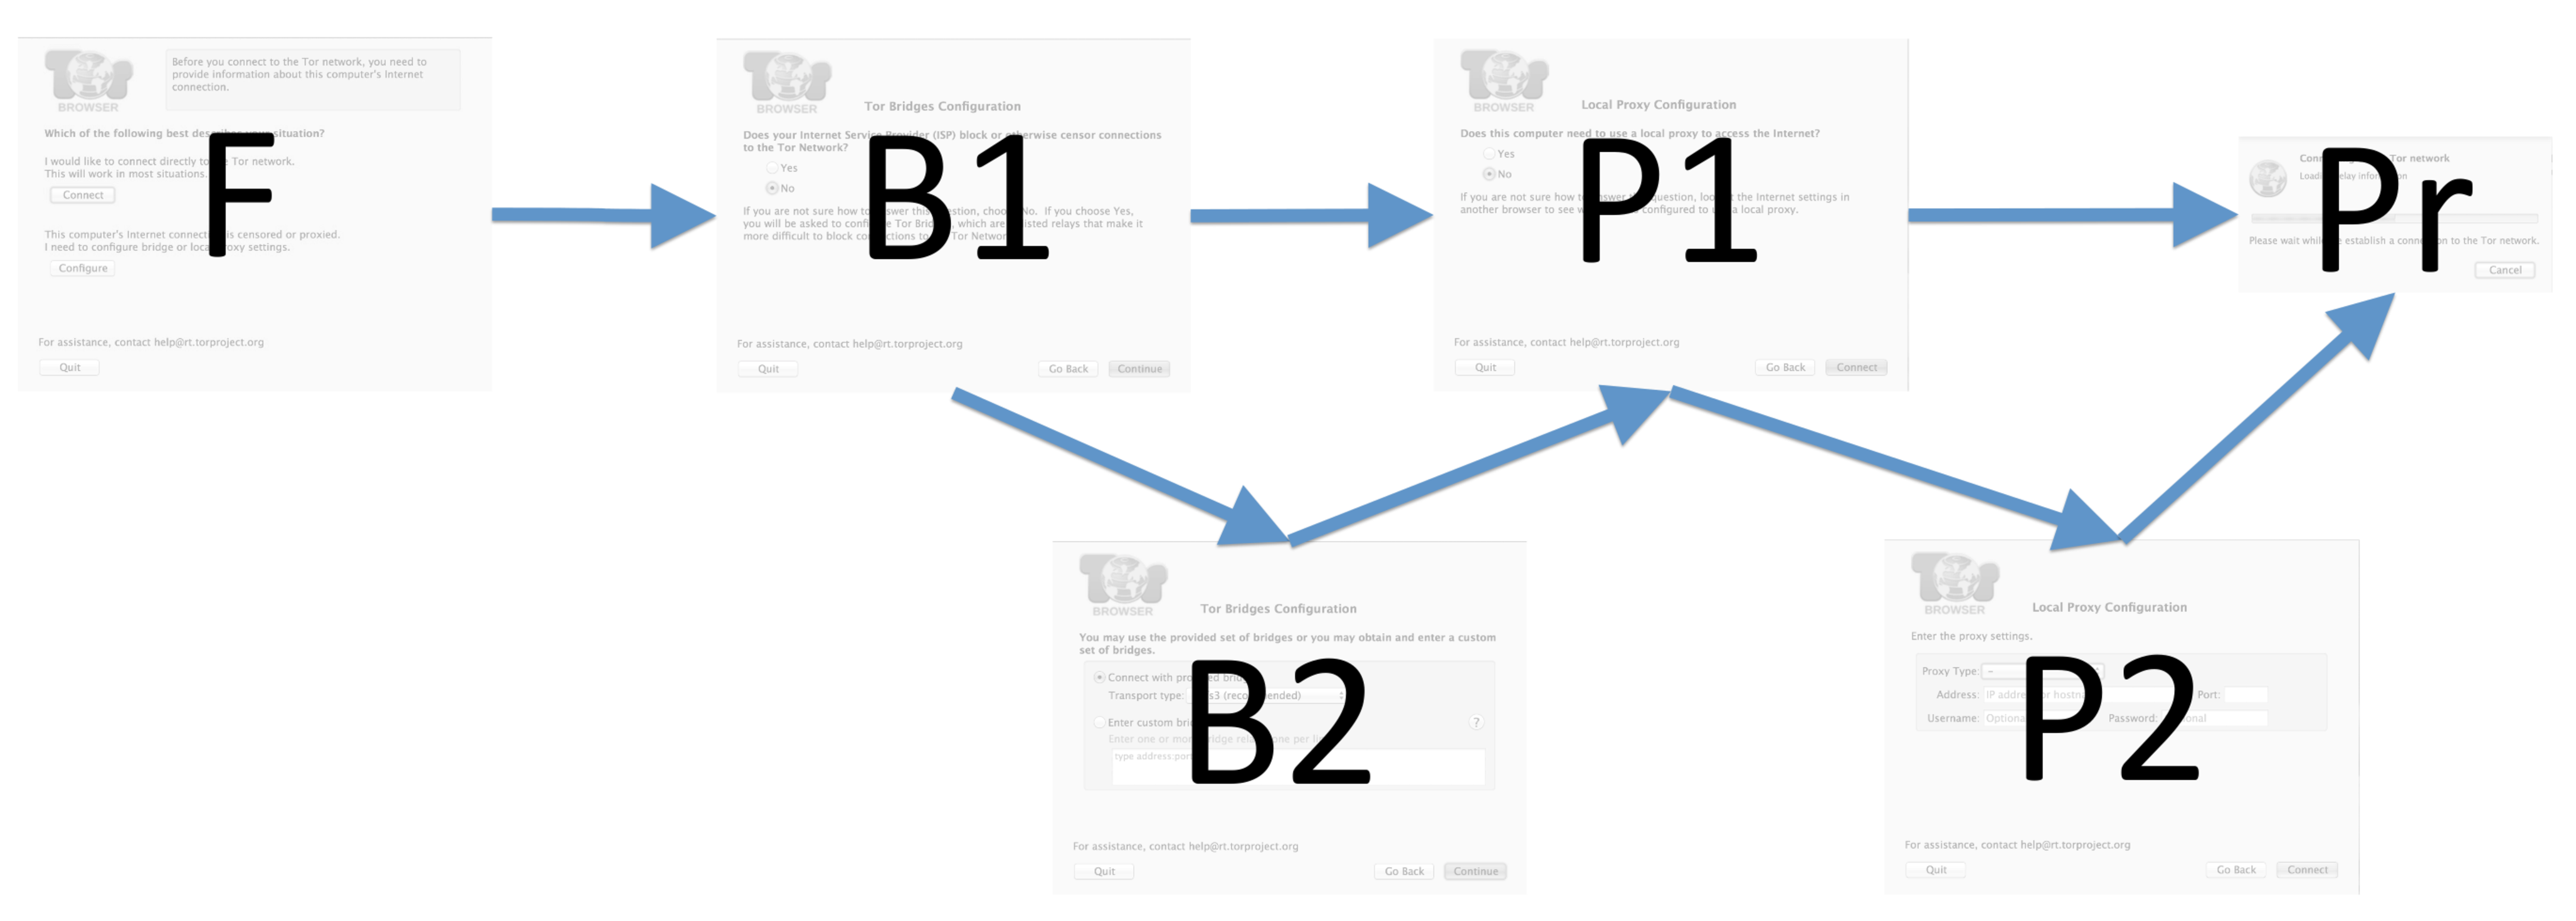
\includegraphics[width=1.0\textwidth]{old-flow.pdf} 
		\caption{old flow} 
	\label{fig:old-flow}
\end{figure*} 

\section{Goals/Evaluation Criteria}
\label{sec:goals}
We evaluate the existing and redesigned Tor Browser configuration interface 
through the empirical evaluation and heuristic evaluation criteria below. The
empirical evaluation criteria were considered during our qualitative and 
quantitative user studies, whereas the heuristic evaluation was considered during
the redesign process. 

A heuristic evaluation is a rule-based evaluation that leverages standards
that have shown to work in the User Interface design 
community. We draw from Jacob Nielsen's ten heuristics~\cite{nielsen1994heuristic}
and other industry standards to form the following heuristic evaluation criteria: \\

\begin{enumerate}
    \item  {\bfseries Visibility of system status}: provide feedback on what the system is doing.
    \item  {\bfseries User control and freedom}: allow users to override system, supports undo and redo actions. 
    \item  {\bfseries Error management}: expressing errors in plain language and offering a solution. 
    \item  {\bfseries Understandable language}: ~6th grade reading level. 
    \item  {\bfseries Minimal design}: suppressing rarely used information to reduce cognitive load. 
\end{enumerate}

Our empirical evaluation criteria for the Tor Browser configuration
interface are from common metrics that measure ease of use with a special 
consideration for high-risk users: \\

\begin{enumerate}
    \item {\bfseries Task Completion}: Almost all can successfully connect to Tor
    \item {\bfseries  Time to Completion}: Time to completion. 
    \item {\bfseries Safe for High-Risk Users}: It should be possible to configure Tor with the interface that it doesn't leak that they are using Tor. 
\end{enumerate}

An exploration of the problems with the existing Tor Browser 
configuration interface through user observation and interviews can be 
found in Section~{\color{red} TODO}. A heuristic evaluation of the existing interface and new interface is in Section~{\color{red} TODO}. We empirically show 
that the redesigned interface improves completion rate, reduces time to completion, 
and provides a safe path for at-risk users in Section~{\color{red} TODO}. 

\section{Qualitative Analysis of the Existing Interface (Study 1)}
We performed qualitative research as an exploratory effort to gain an 
understanding of underlying problems, such as reasons for confusion 
during the configuration process and motivations for particular choices in 
configuration. We did this through observing each participant as they 
interacted with Tor Browser 5.0.3 interface and interviewed them about
their experience. This study provides insights into particular problems with 
the current Tor Browser configuration interface, and helps us to design
a new interface which addresses these problems and gives foundation
for hypotheses to test in quantitative research. 

\subsection{Methodology} 
In this section, we talk about the details of our qualitative user study, such as the inspection of the interface, censorship environments we placed our users in, how we pre-screened and selected our participants, and the procedure for the experiment. 

\subsubsection{Inspection} 
A combination of usability inspection methods~\cite{nielsen1994usability}
 were used prepare for the user study. Two researchers conducted a pluralistic 
walkthrough and stepped through various censorship
scenarios, discussing which elements would be involved for that use case, and walking 
through the configuration process. After compiling all the possible paths through the 
interface {\color {red} digraph here?}, feature inspection was performed to list sequences
of features used to accomplish typical tasks, taking note of long sequences or cumbersome
steps. To focus our observations, a heuristic evaluation was performed to mark design issues 
that may cause confusion for users during our study. 

\subsubsection{Setup}
\label{sec:setup}
We simulated three censorship environments for our experiment.
These reproducible, stable environments are informed by our experience 
with pluggable transports and knowledge of commonly seen censorship 
techniques. Their goal in our user study is not to replicate the network 
environment in any particular country, but to require our participants to 
configure Tor Browser in distinct configurations. \\

\begin{itemize} \itemsep1pt \parskip0pt \parsep0pt
\item {\bfseries Mild censorship (E1)}: 
(Representative of countries such as France and Australia.)
Certain domains are blocked. Reaching these 
domains requires a censorship circumvention 
tool. The default option to ``connect'' to the Tor network 
directly will circumvent this censor. Additional correct
bridge or proxy configurations are optional. 

\item {\bfseries Intermediate censorship (E2)}: 
(Representative of countries such as Tunisia.)
Certain domains are blocked. Censorship circumvention
tools such as Tor are blocked. Since all public Tor
relay nodes are blocked, the default option to ``connect'' to the Tor network
directly will fail. Any choice of a hard-coded bridge
or a valid non-public bridge will circumvent this censor.  
Additional correct proxy configuration is optional.

\item {\bfseries Comprehensive censorship (E3)}:
(Representative of countries such as China and Syria.)
Certain domains are blocked. Censorship circumvention tools
are thoroughly blocked. Tor is blocked by blocking all public
Tor relay nodes, and the censor has examined source code to block
all hard-coded bridge relays in the configuration interface. The default option
to ``connect'' to the Tor network directly will fail. Most bridges will fail,
but ``meek-amazon,'' ``meek-azure,'' and ``meek-google'' still work.
This is because domain-fronting requires censors to block entire CDNs to also
block this transport (which will cause huge collateral blocking damage), making
it resistant to aggressive censorship environments.
(See ~\cite{fifield2015blocking} for additional details.)\\
\end{itemize}

\subsubsection{Recruitment}
Using established best practices from the field of user experience research~\cite{howmanyusers},
we recruited 5 participants for each censorship environment.
We pre-screened ~\cite{screening} our participants for diversity of gender, age, technical expertise,
and familiarity with Tor in each simluated censorship environment for our summative
usability test~\cite{summative}. 

We recruited our users from Craigslist. The recruitment text can be found in 
Appendix~\ref{qualitative-recruitment}. The recruitment posting contained a 
SurveyGizmo online survey that collected information about our participants.
The complete prescreening survey can be found in Appendix~\ref{qualitative-prescreening}.  

We chose our participants based on the pre-screening information to have 
at least one person who has never heard of Tor, at least one person who has 
only heard of Tor, and exactly one person who has previously used Tor in each
environment. We also tried to evenly distribute any participants who had technical
expertise or used particular security tools throughout the censorship environments. 

Out of our 16 participants, ages ranged from {\color {red} TODO}
(sigma = {\color {red} TODO}). {\color {red} TODO} of our participants had at least
a college education, and the most common jobs included {\color {red} TODO} and
{\color {red} TODO}. {\color {red} TODO} had heard of Tor previously, 
and {\color {red} TODO} had used Tor previously. {\color {red} TODO} out of 
16 did not use any circumvention tools, and no more than {\color {red} TODO} 
knew any more than {\color {red} TODO} technological terms.

\subsubsection{Procedure}
We conducted a qualitative evaluation of the interface by creating an environment 
for users to interact with the configuration interface in a censored environment, 
observing their interactions in real time without interacting with the participants, 
and following up with interviews about their experiences.

The one-hour, single-participant procedure begins when a participant enters a small 
room with a single computer, which is equipped with Tor, Chrome, Firefox, Internet Explorer, 
Chrome, and VLC (for screen recording). A participant is firstly informed of 
the risks of the study and consenting to data collection. If they consent, the 
experiment begins. A researcher informs the participant that they are in a
simulated censorship environment, where some websites and services are blocked. 
For the full script of what participants have heard, see Appendix~\ref{qualitative-script}. We
instruct them to visit a sample blocked website and a sample non-blocked website on a
non-Tor browser of their choice to illustrate the situation.

After illustrating the censorship environment, participants are asked to 
complete a worksheet that asks to visit one blocked website and one non-blocked website. 
We chose Wikipedia's featured article of the day as the blocked website and 
the CNN homepage as our non-blocked website because the familiarity 
that most users have with these websites makes the browsing task relatively easy, 
which focuses participants' attention to configuring Tor Browser. 

After instructions, researchers stepped out of the room so that there was no interaction
between the participant and researcher for the rest of the session. Participants' screens 
were recorded and streamed to another room, where the researchers were able to 
observe how a participant configured their browser. Participants had an 
average of 45 minutes to complete their worksheet. 
At this point, the participants do not know the details of their censorship environment,
only that they are actively being censored. We believe that this is representative 
of the mental model of users in censored countries, and therefore chose to simulate 
this for the experiment. Ultimately, participants needed to configure Tor Browser to 
circumvent the simulated censorship. 

After users completed the browsing tasks or have spent the rest of the time
trying to configure Tor Browser, we interviewed participants about their experience.
We performed a live transcription of the interview to avoid recording voices, which is
considered personally identifying information. 
We asked three standard questions asking about their general experience, 
confusing interface features, and soliciting feedback for improvements. We followed up
with specific questions we had for a particular participant from observing their screen. 
This was to verify any hypothesis we had about the participant (i.e. ``they didn't know what to do on window~3'').  
After their interview, participants were informed that the experiment was over and 
given their payment of~\$30. 

\subsection{Results} 
In this section, we discuss problems encountered by our participants at each step of the configuration process and solutions to those problems. We conclude with our goals for improving the configuration interface. Because of the small sample size of qualitative studies, we can only state that these are problems that participants can encounter when configuring. We confirm the statistical significance of some of the problems in our quantitative study (Section~\ref{sec:quantitative}). All quotes are paraphrased from live transcriptions of participant interviews.\\

\subsubsection{Connect vs. Configure} 
The first task for our participants was to decide between connecting directly to the Tor network or configuring their connection. Text in the interface tells people that connecting directly ``will work in most situations'' and instructs to configure a bridge or proxy if the ``Internet connection is censored or proxied.'' We found that a majority of our participants did not take the time to read the text on the screen and that if they did, the text did not always soundly influence their decision.

The participant across all censorship environments connected directly to the Tor network. When they did, they did so because they were taking the path of least resistance first or intimidated by the configuration process. 
\begin{quotation}
\noindent P9: \textit{``Configure seemed manual, so I clicked connect.''}\\

\noindent P14:\textit{``The words were confusing. I don't really understand computers. I don't know what configure means in this setting. Hmm, is it going to crash? When you see connect, you want to click it because you really want it to connect.''} 
\end{quotation}

Bridges are only necessary when Tor relays are censored, but participants are not able to determine when this happens, or what the difference between a blocked website and a blocked relay looks like. Participant 10 and several other participants in the mild censorship environment opted to configure a connection when a direct connection to the Tor network would have worked. 

\begin{quotation}
\noindent P10: \textit{``I was censored, so I picked the configure.''}
\end{quotation}

This mistake can result in users struggling through the rest of the interface similarly to those in the intermediate and advanced censorship environments.
% FIXME:
Participants in the intermediate and advanced censorship environments who did correctly choose to configure in intermediate did not actively display an understanding between the difference between censorship of websites versus censorship of the Tor relays.

Making the choice between connect and configure clearer for users has the possibility to save time and keep users safer. Waiting for a failed connection takes about couple minutes, so users can save at least that time by making the correct decision the first time. Users who need to configure can benefit from not clicking connect, which keeps them safer by not leaving a detectable network trace that indicates that they are trying to use Tor to circumvent censorship.\\

\subsubsection{Bridge Configuration} 
When a participant chooses to configure their connection, their next step is to determine whether they need to configure a bridge, and to configure one if necessary. Answering yes to ``Does your Internet Service Provider (ISP) block or otherwise censor connections to the Tor Network'' directs to a bridge configuration screen, whereas answering no skips that screen. We observed that multiple participants struggled with the technical language on the screen, and ultimately decided to try trial and error. Most participants with the default option to not configure a bridge. 

\begin{quotation}
\noindent P7:\textit{``The bridge screen was the most challenging. It seemed very technical to me. I don't know what a bridge is.''}\\

\noindent P12:\textit{``I decided which options to choose by process of elimination with trial and error.''}
\end{quotation} 

On the bridge configuration screen, participants need to choose between configuring a built-in bridge versus a custom bridge. Participants were unsure of the difference between a built-in bridge and a custom bridge and also why one would use a custom bridge. Most participants chose to go with the built-in bridge and chose obfs3 as their transport, because those were the default options on the screen. 

\begin{quotation} 
\noindent P8:\textit{``I have no clue what's the difference between flashpoxy, fte, etc. I need to know why the built-in ones aren't working. And why do I need a custom bridge if there are options built in?'}\\

\noindent P7:\textit{``Since it (obfs3) said recommended, it helped actually, and I selected it because it was chosen. I saw the custom bridges option, but I didn't know what to enter there so I went with this (obfs3).''}
\end{quotation} 

Participants in the advanced censorship environment were required to select a meek bridge (not the default) or to configure a custom bridge. After the first pluggable transport failed and if the participants deduced that the source of the failed connection was a mis-configured bridge, the pluggable transport names only confused participants and caused odd behaviors. Participants chose bridges in every order imaginable: at random, in order of the list starting from the default, in order of the list starting from the top, at random, choosing accessible sounding names first (i.e. meek-amazon over fte), and choosing non-accessible sounding names first (i.e. fte over meek-amazon). 

\begin{quotation}
\noindent P4:\textit{``When I saw obfs3 as the recommended option, the next option logically for me was obfs4.''}\\

\noindent P5:\textit{``I tried the pluggable transport that used google, because I noticed that google was working (when I was using a non-Tor browser).''}
\end{quotation} 

Providing explicit guidance on in which order participants should try the bridges will be critical in helping a user succeed in configuring their connection. Rather than letting the user choose, the interface can guide the users by telling them to choose specific bridges if the default doesn't work, and in what order. Our participants were resilient in trying to configure a connection for up to 40 minutes, but we believe that this is a byproduct of the experimental setting and compensation. \\

\subsubsection{Proxy Configuration} 
After the bridge configuration, the participant again is asked to answer a question to determine if they need a proxy and if so, to configure one. This question also was too technical for some participants.

\begin{quotation}
\noindent P11:\textit{``I think you can only answer this question (does this computer need a local proxy) if you know what a local proxy is. Otherwise, you have no chance..''}
\end{quotation}

All who chose to configure a proxy were successful. Many of the participants followed the directions in the interface to look at the Internet settings in another browser to see whether it is configure to use a local proxy, but they never found the proxy information since none of the other browsers had the information. What further frustrated the situation was that the other browsers did not explicitly state that no proxy was configured, which caused many of our participants to search for proxy settings.

None of our censorship environments required our participants to configure a proxy for a successful connection. Upon the first attempt at configuration, most chose the default value of not configuring a proxy. However, trying to unsuccessfuly configure a proxy was the most common reason for failing to connect. Since the interface passively re-displayed a proxy-related window seen after an attempted connection regardless of the error, many participants were convinced that they needed a proxy to connect to the Tor network. Users did not check their incorrect assumption ~\cite{wason1960failure}. This false assumption can be fixed by giving information on what needs to be configured~\cite{reeder2005user}. \\

\subsubsection{Progress Bar} 
Users were generally displeased with the lack of feedback on the progress bar. Users do tolerate delays if they are for security reasons, but only to a certain extent and if they understand the security reason ~\cite{egelmanplease}. Participants in our study usually did not understand the security reason, and experienced huge delays on the order of minutes, even in the ideal case in which a user chose the correct configuration in the first attempt. If users chose particular wrong configurations (i.e. a syntactically valid but nonfunctional proxy), they would be waiting for an indefinite period of time, because there is no timeout. 

\begin{quotation}
\noindent P16:\textit{``There doesn't seem to be a timeout on any of this stuff. Am I waiting long enough? It should work immediately.''}\\

\noindent P6:\textit{``How long does this actually take (to connect)? This took way too long, and I didn't know how long it should take.''}
\end{quotation}

As a technical artifact of how the progress bar is implemented, the progress bar remains empty on subsequent attempts to connect to the Tor Network until the percent progress supersedes the last displayed progress value (i.e. a participant who saw 30\% progress on their first attempt would see 0\% progress in the progress bar until subsequent attempts got at least 40\% progress). The negative feedback of a 0\% progress bar would cause users to assume that their subsequent attempts were wrong, even if they were correct. 

\begin{quotation}
\noindent P1:\textit{``It was hard to figure out if the progress bar wasn't moving because the connection was censored, or if it was just slow.''}
\end{quotation}

Ensuring that the progress bar faithfully displays the current status can encourage users to wait for correct configurations to successfully connect to the Tor network. 

\begin{quotation}
\noindent P15:\textit{``I didn't know if this computer had any proxy information. I wasn't able to find it if it did.''}
\end{quotation}

Providing participants with feedback about taking specific actions (such as trying a different bridge, trying the same configuration again, try connecting directly, etc. can prevent participants from unnecessarily configuring a proxy and to connect successfully.\\

\subsubsection{User Communication} 
Many participants, including participants who were pre-screened for high technical ability and previous experience with using Tor, were not familiar with the vocabulary. 
\begin{quotation}
\noindent P2:\textit{"I don't know what any of those means (list of bridges),or what that (proxy)
 means at all."}\\
 
 \noindent P3:\textit{``The vocabulary is really challenging, for someone not doing IT work.''}\\
 
 \noindent P4:\textit{``The progress bar had no feedback for me. I didn't know why I was getting back `establishing encrypted directory'--what does that mean?''}\\
 
 \noindent P16:\textit{``Because I never configured a proxy or worked with that stuff, I was just going to keep clicking and pray.''}
\end{quotation} 
In addition to the text being not as helpful as it would have been had users been able to understand, this discouraged our users during the process. Communicating the relevant information in an understandable way is difficult, bu is critical for the usability of a system ~\cite{molich1990improving}.\\

%\begin{quotation}
%\noindent{\bfseries P15}:\textit{``Give this to a couple of people who know how to do this. They can feel elite\ldots they only want the elite to use some computer things..''} \\
%\noindent{\bfseries P13}:\textit{``I don't remember what I did. I figured it out? What? <laughs> Oh man, that's crazy..''}\\
%\noindent{\bfseries P11}:\textit{``Is this question (does your ISP censor your Internet connection) really necessary? I just selected that I have a censored connection, why do they ask me again?''}
%\end{quotation}

\section{Redesigning the Configuration Interface}
%skip talking about the process of redesigning the interface. It isn't that interesting. 

% Heuristic evaluation metrics, from above: 
% \begin{enumerate} \itemsep1pt \parskip0pt \parsep0pt
%     \item {\bfseries Visibility of System Status} provide feedback on what the system is doing.
%     \item {\bfseries User Control and Freedom} allow users to override system, supports undo and redo actions. 
%     \item {\bfseries Error Management} expressing errors in plain language and offering a solution. 
%     \item {\bfseries Understandable Language} ~6th grade reading level. 
%     \item {\bfseries Minimal Design} suppressing rarely used information to reduce cognitive load. 
% \end{enumerate}

Tor Browser 5.0.3. configuration interface does not adequately meet our heuristic evaluation criteria from Section~\ref{sec:goals}: visibility of system status, user control and freedom, error management, understandable language, and minimal design. The configuration used for a connection is not visible to the users before they connect or while they are connecting, full control but little guidance through the configuration process confuse users, error messages do not express errors in plain language nor offer solutions, the text was too technical for an average user to understand, and the interface has room to be simplified visually.  

Currently, the interface overburdens users. Our goals in redesigning the interface was to making the system status visible to the user, retain user freedom but give guidance, make the vocabulary more accessible, offer solutions upon errors, and to require the user to make fewer decisions overall. To achieve these goals, we made the following changes: \\

\begin{figure*}[t]
	\centering
		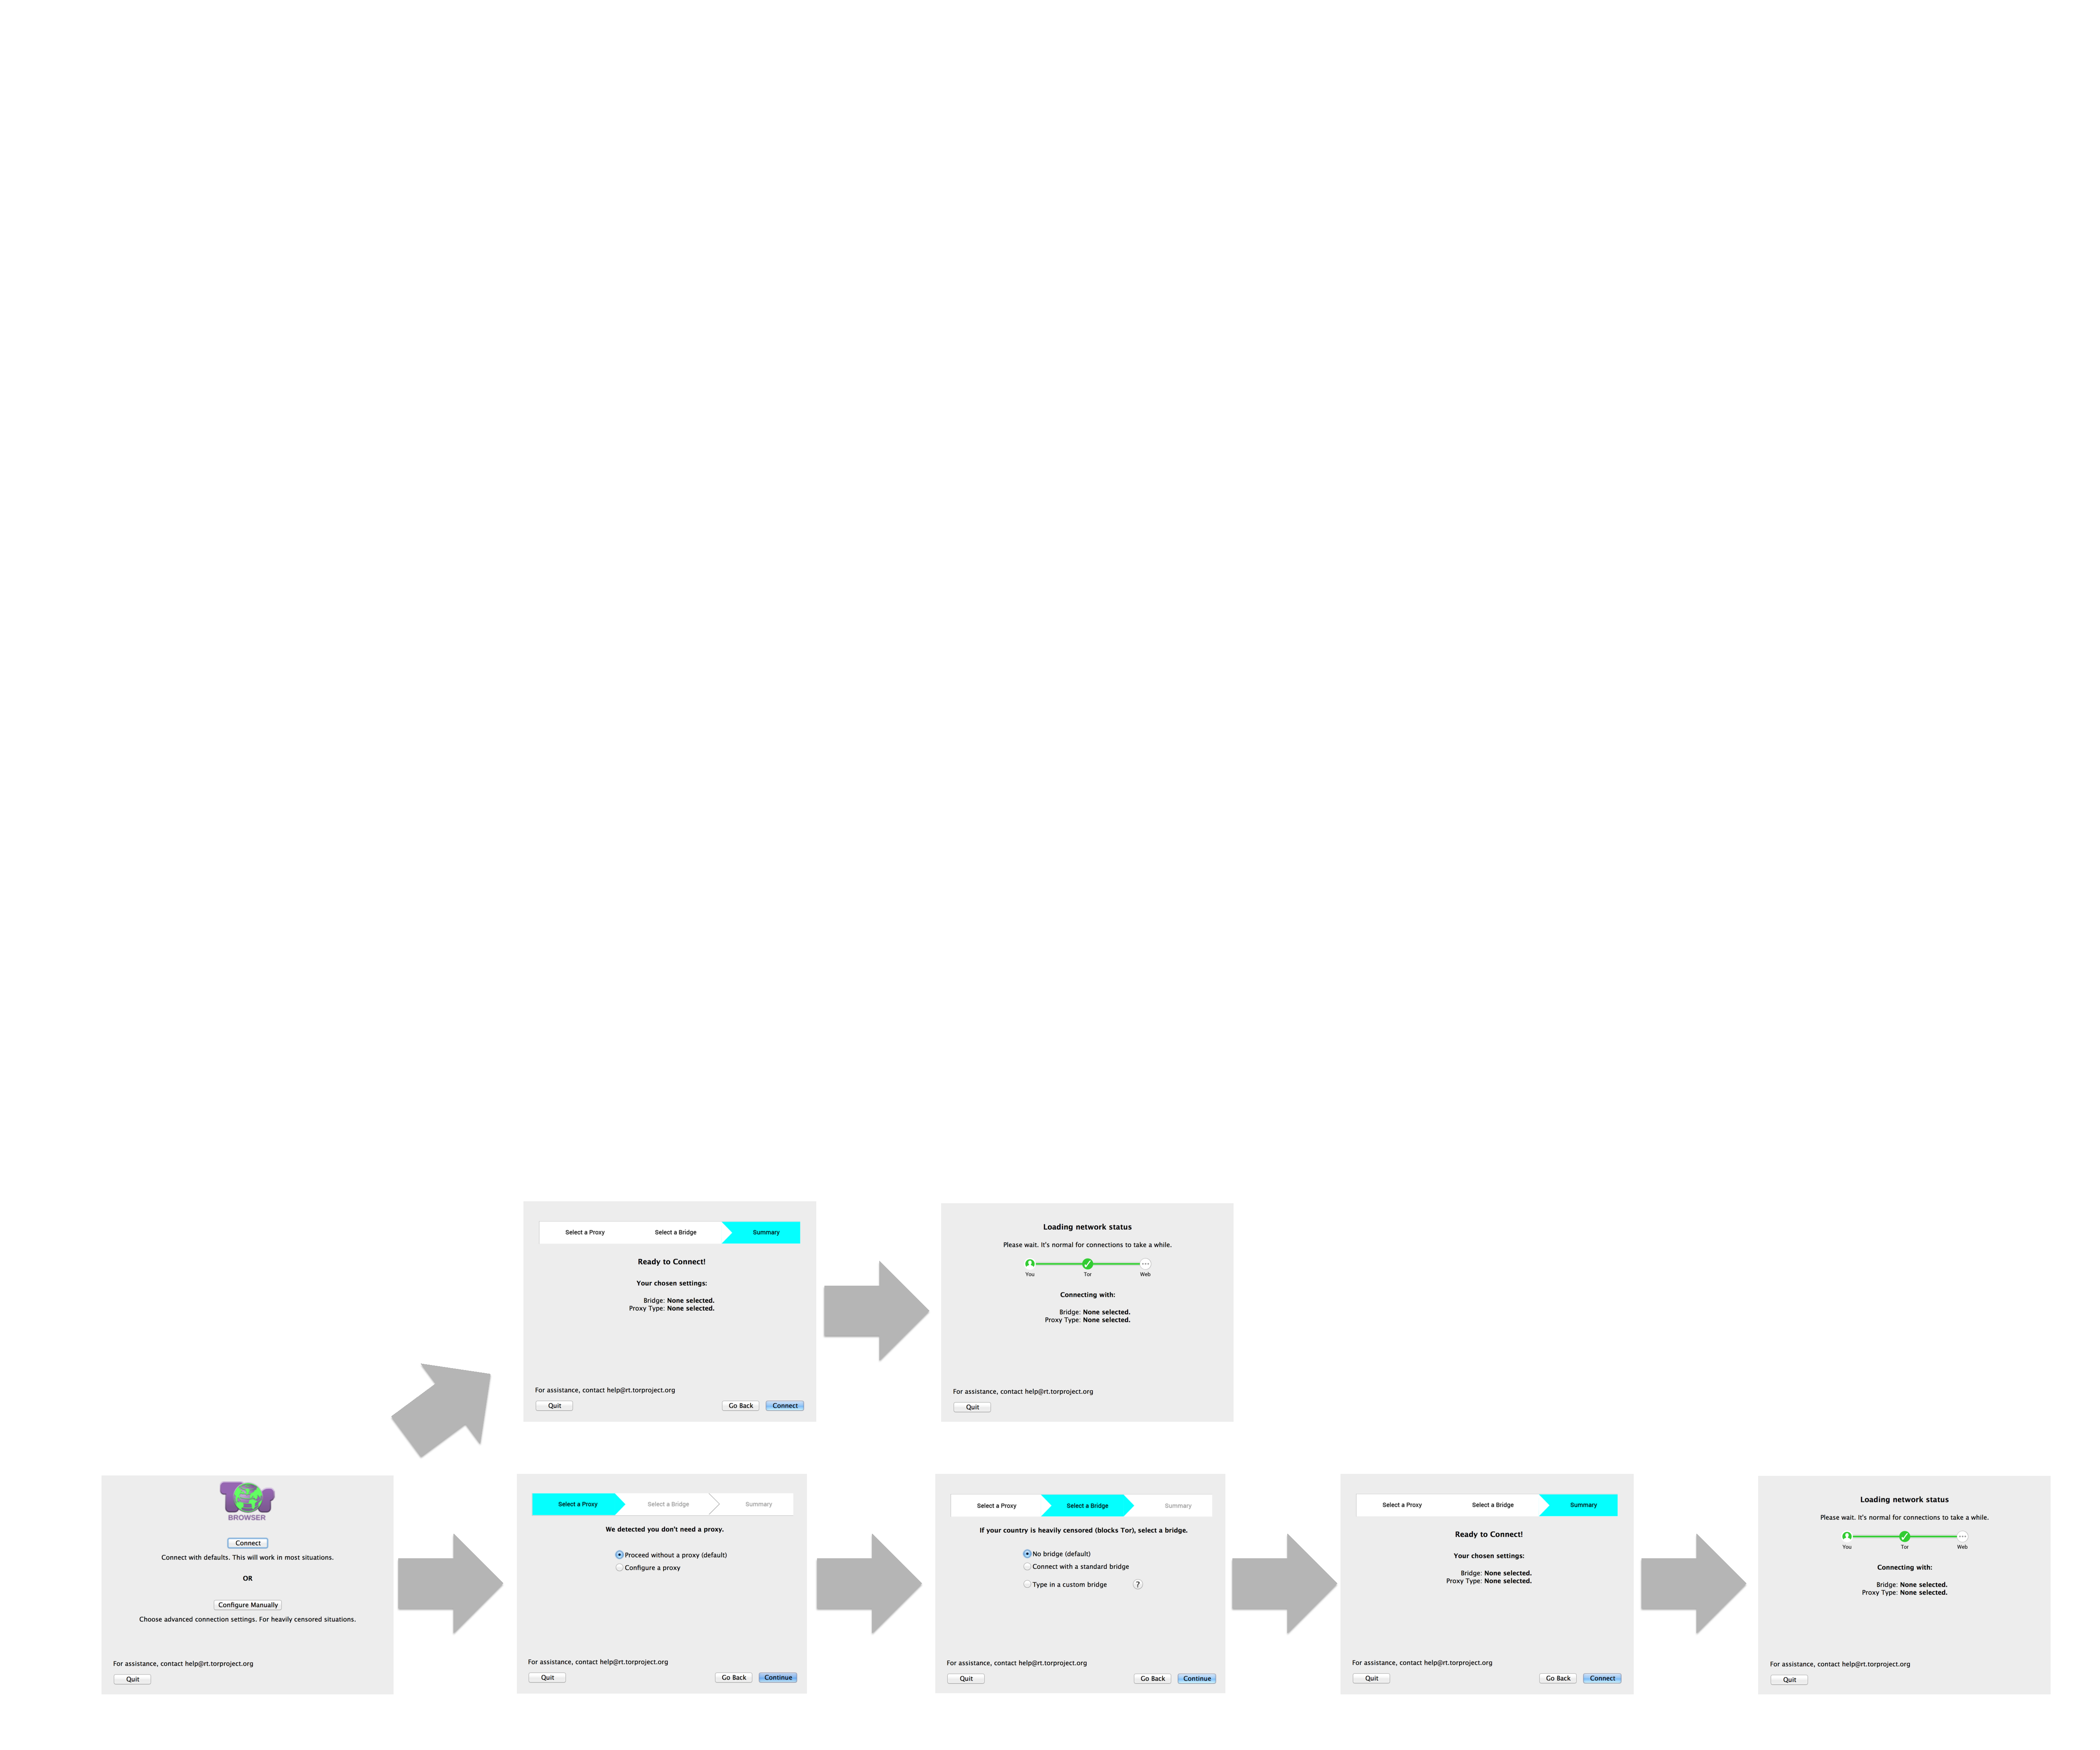
\includegraphics[width=1.0\textwidth]{new-flow.pdf} 
		\caption{new flow} 
\end{figure*} 

\begin{figure*}[t]
	\centering
		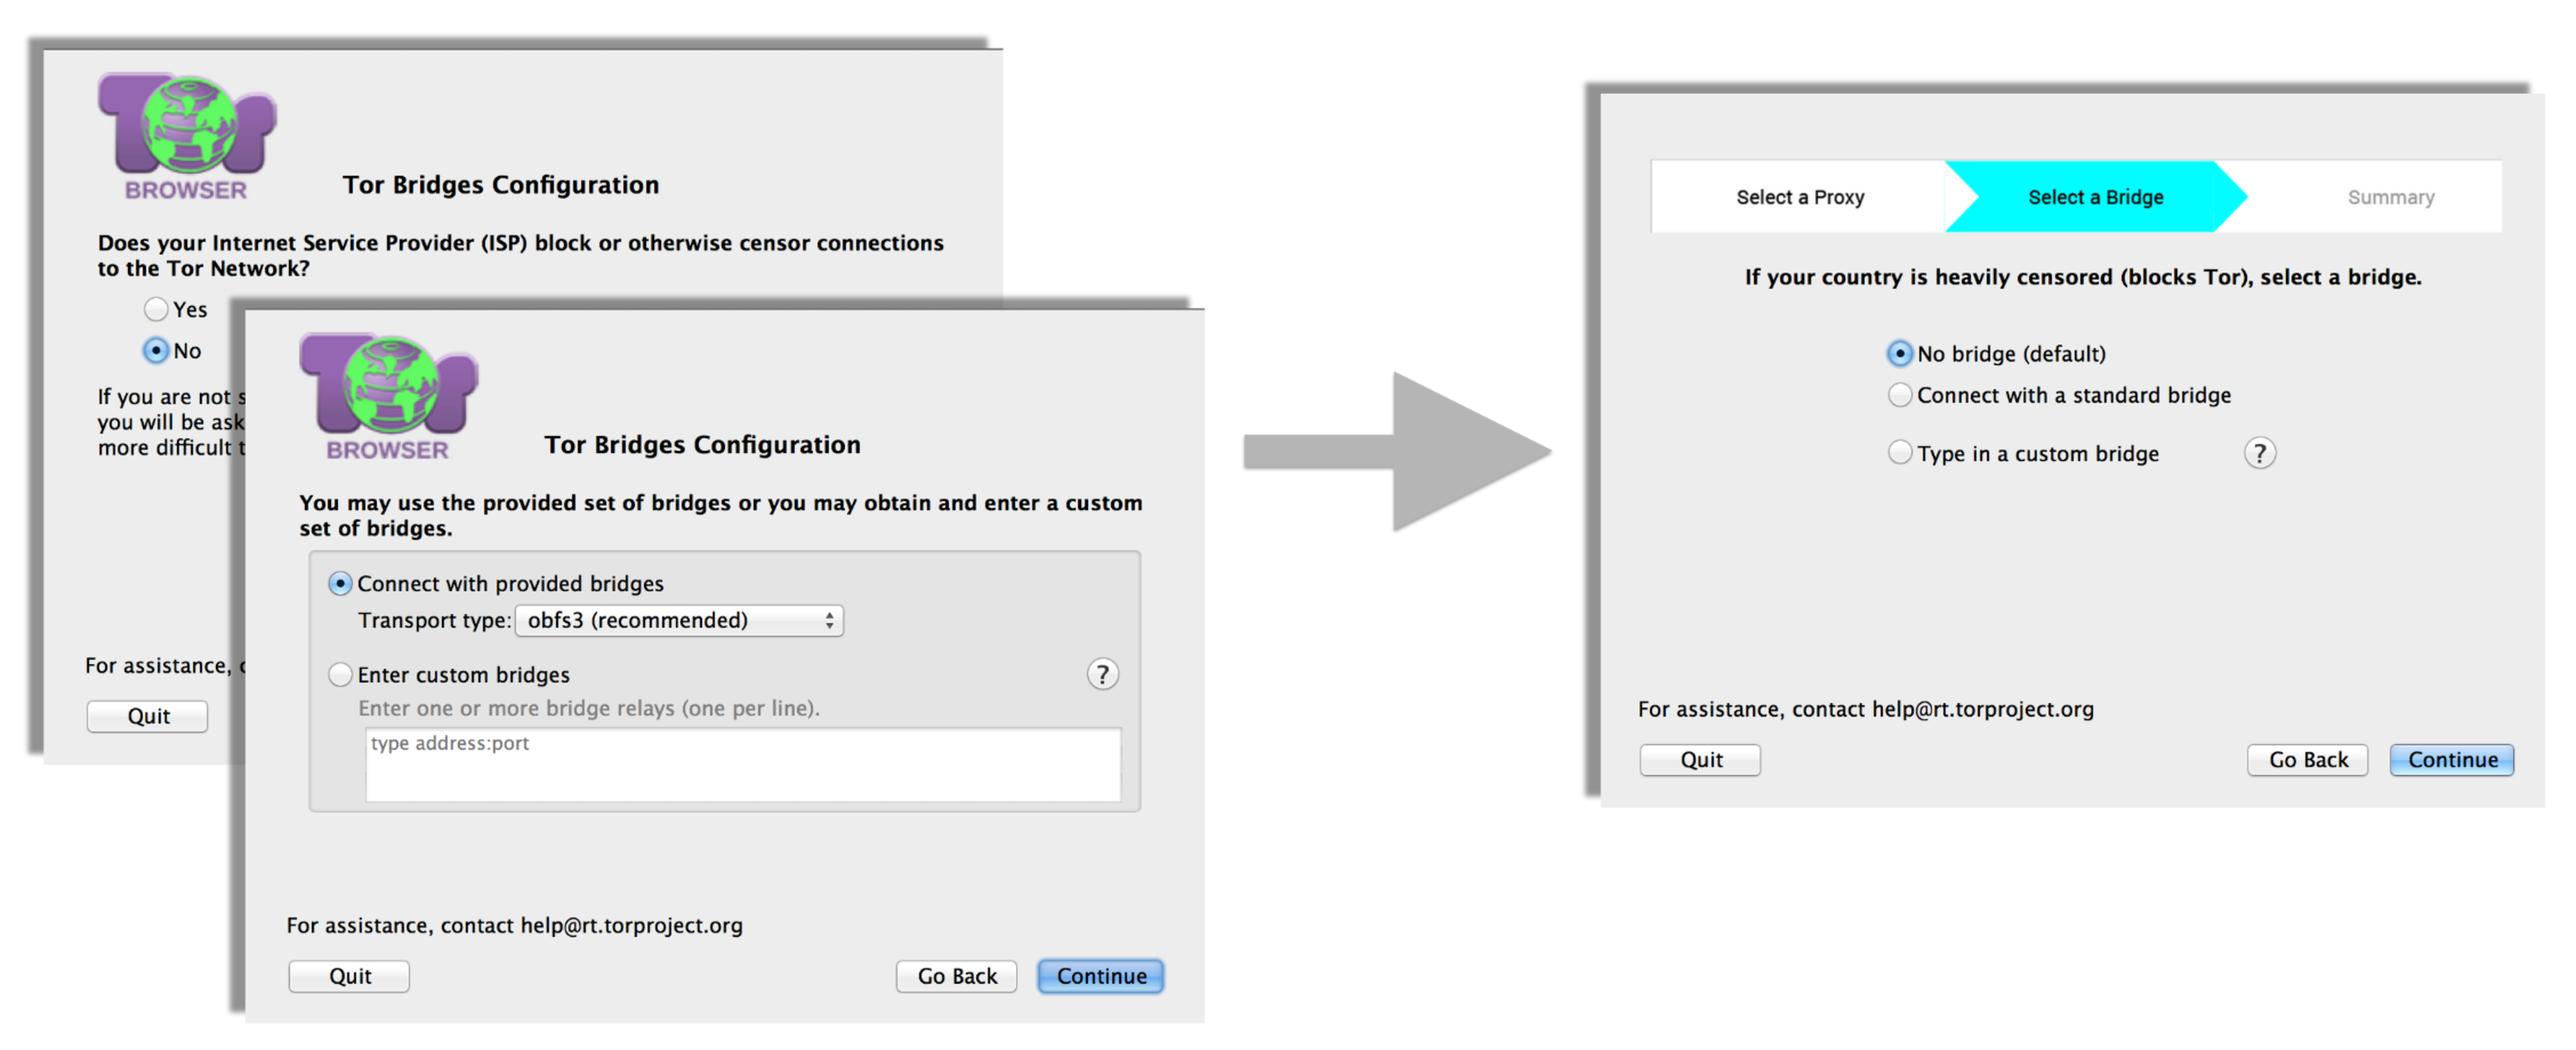
\includegraphics[width=1.0\textwidth]{bridge-screens.pdf} 
		\caption{bridge screens} 
\end{figure*} 

\begin{figure*}[t]
	\centering
		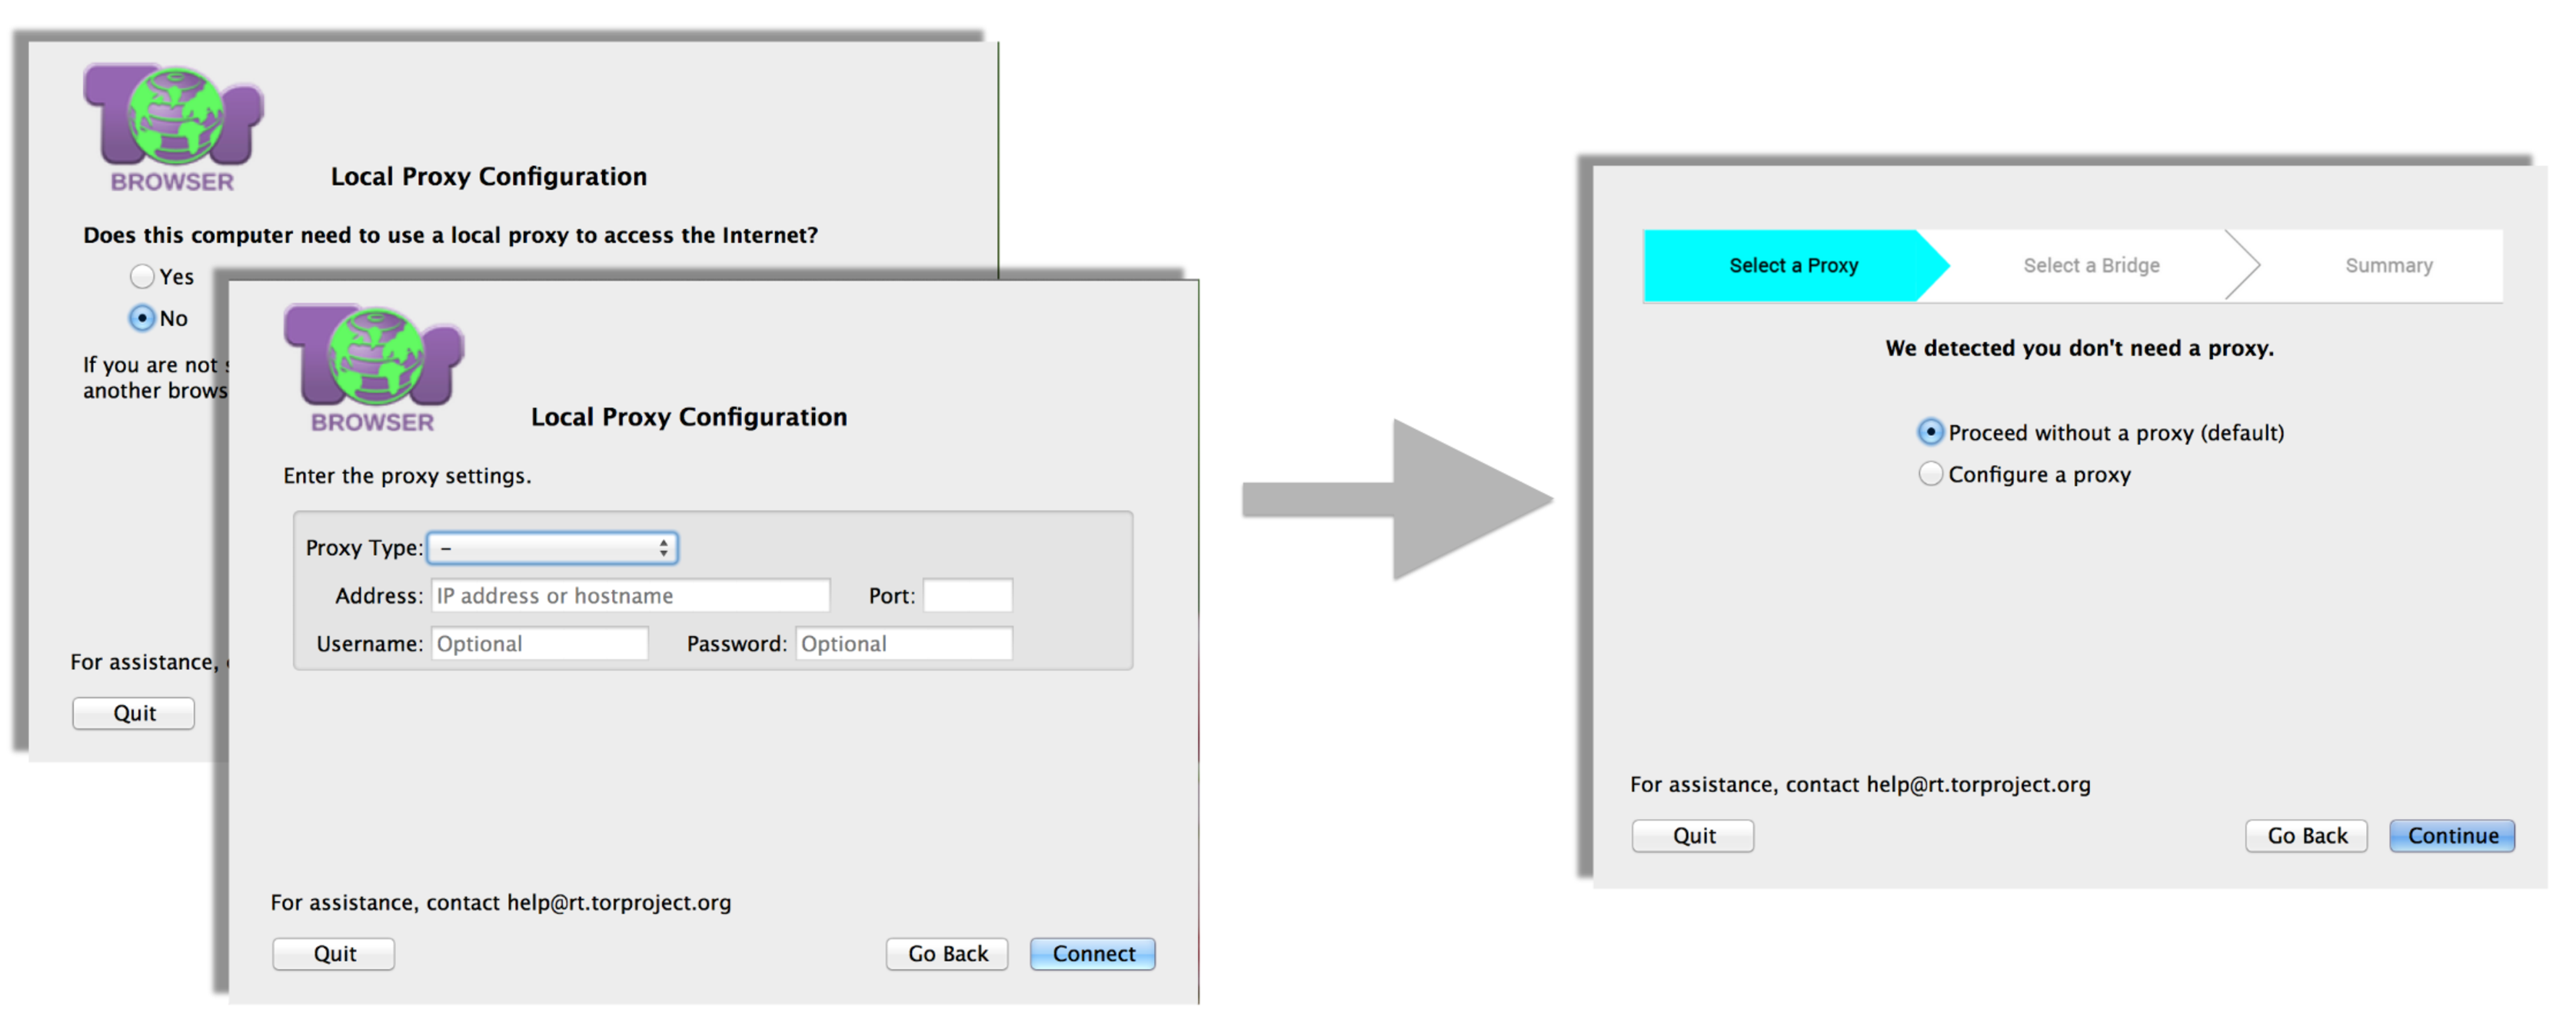
\includegraphics[width=1.0\textwidth]{proxy-screens.pdf} 
		\caption{proxy-screens} 
\end{figure*} 

\begin{enumerate} \itemsep1pt \parskip0pt \parsep0pt 
\item {\bfseries Added system status visibility.} Before any attempt to connect to the Tor network, a summary screen displays if a bridge or proxy is configured, and if so, what the configurations are. The progress screen also displays the configurations while the connection attempt is being made. 
\item {\bfseries Added guidance on choosing connect vs configure.} We labeled the configure option as advanced, manual, and only for heavily censored situations. 
\item {\bfseries Got rid of proxy and bridge questions.}  We removed the bridge and proxy questions, which were highly technical and challenging for users to answer. There are two less windows in the interface.
\item {\bfseries Added auto-detect for proxies.} Auto-detection of proxies can be done locally, by scanning system files. This is safe even for at-risk users, and greatly simplifies the configuration process. 
\item {\bfseries Switched ordering to configure proxies first.} To build up the users' mental model, we configure network components in a topologically sequential. Proxies were put after bridge configuration because only a small fraction of users require proxies. With auto-detection, configuring a proxy before a bridge will not burden the users. 
\item {\bfseries Added explicit advice on choosing bridges.} The default bridge is still obfs3. There is added text that advises users to try a meek bridge if obfs3 does not work. This advice is tailored for our participants who were in the advanced censorship environment. 
\item {\bfseries Added more feedback to the progress bar.} The progress bar shows network components involved in connecting to the Tor network and gives feedback to the user as they are correctly configured. For instance, a user can can now see that the bridge was configured correctly, and they just need to wait to connect to the Tor network. Upon failure, users can see which components that have succeeded and which have failed. 
\item {\bfseries Added instructions on what to try next on errors.} When an error occurs, advice on what to try next is shown to the user. Such advice includes trying the connection again, choosing a different bridge, or trying a connection without a proxy. 
\item {\bfseries Reduced overall amount of text and made text less technical.} We make the text more accessible by focusing on instructing users through the configuration process, at the sacrifice of explaining technical concepts to users. Since users generally couldn't understand the technical concepts enough to influence their decisions, giving direct guidance may be a better option.  
\item {\bfseries Reduced visual clutter.} Whenever we could, we minimized the amount of text on the screen, hid additional fields until the relevant options were chosen, and made additional stylistic simplifications. 
\end{enumerate} 

The redesigned interface maintains the approach taken by the deployed interface of asking the users about their situation, which is in the spirit of the deployed interface. The designed interface conservatively interacts with users by automating only safe configuration processes and still allowing users to have control over configuring all interacting network components. The design requires more maintenance because of the explicit advice given on which order to select bridges and advice on error messages, which may change as the censorship environments change. For additional changes that can be made and alternate approaches for interacting with the user, see Section~\ref{sec:discussion}. 

\section{Quantitative Analyses of the Interfaces (Study 2)}
\label{sec:quantitative}
We performed quantitative research to quantify the existing problems
and the impact of our redesign by generating numerical data to transform
into usable statistics. Specifically, we collected all events, transitions, 
and state for Tor Browser 5.0.3 and the redesigned Tor Browser. Participant
logs of how they interacted with each of these interfaces are used to both
quantify the issues we encountered in our previous qualitative 
study and to examine the differences in success rate, time to completion,
and configuration choices between the two versions. 

\subsection{Methodology} 
In this section, we talk about the details of our quantitative user study, such as the censorship environments we placed our users in, how we recruited our 124 participants, and the procedure for the experiment. 

\subsubsection{Setup}
For consistency, we simulated the same three censorship environments from 
our qualitative user study. Details of the mild, intermediate, and advanced 
censorship environments and what configurations are necessary for a 
successful connection can be found in Section~\ref{sec:setup}. 

We prepared special instrumented versions of both versions of Tor Launcher.
The instrumentation logs recorded every meaningful interaction with the interface---every
button press, every menu selection, every screen change---along with a timestamp.
The logs enabled us to calculate statistics such as the success rate
for each condition.

We recorded a video of the contents of the computer screen throughout each session.
Review of the videos revealed details not captured by the instrumentation logs alone,
such as participants' web searching and inspection of system networking settings.

\subsubsection{Recruitment}
We recruited 20 users for each censorship environment
and interface combination, resulting in a total of 120 users. This decision 
was due to both data analysis considerations (large enough to have good effect size, 
with a minimum of 20 to be able to assume normal distributions) and
available funding.

We recruited half of our users from Craigslist, and half of our participants from 
the Xlab participant pool. It is standard for Xlab experiments to be run with Xlab
participants, who have been verified of their identity and have good attendance
rate. Although Xlab participants are not limited to UC Berkeley students and staff,
a majority of the participants are from campus. For this reason, we chose to recruit 
half of our participants from Craigslist to ensure a diverse set of participants. 
The recruitment text can be found in Appendix~\ref{quantitative-recruitment}. 

We chose our participants on who had responded to our listing first and their
availability for experiment sessions. We collected their demographic information
with an exit survey that participants took after the experiment. 

Out of our {\color {red} TODO} participants, ages ranged from {\color {red} TODO}
(sigma = {\color {red} TODO}). {\color {red} TODO} of our participants had at least
a college education, and the most common jobs included {\color {red} TODO} and
{\color {red} TODO}. 

\subsubsection{Procedure}
Similarly to the qualitative experiment, we conducted a quantitative evaluation 
of the interface by creating an environment  for users to interact with the 
configuration interface in a censored environment. The focus of this environment 
was to collect a dataset of metrics to evaluate the two interfaces. 

The one-hour, multi-participant procedure begins when all participants are sitting at their
respective computers in Xlab. Each computer is equipped with an old or modified version
of Tor Browser, Chrome, Firefox, Internet Explorer,  Chrome, and VLC (for screen recording). 
Participants are firstly informed of the risks of the study and consenting to data collection.  At
this time, participants are given the chance to leave the laboratory if they do not consent to 
the experiment conditions. When every participant left in the room has turned in their consent
form, the experiment formally begins. A researcher informs the participants that they are in a
simulated censorship environment, where some websites and services are blocked. 
For the full script of what participants have heard, see Appendix~\ref{quantitative-script}. We
instruct them to visit a sample blocked website on a non-Tor browser of their choice to illustrate 
the situation.

After illustrating the censorship environment, participants are asked to 
complete a worksheet that asks to visit one blocked website. 
Similar to the qualitative study, we chose Wikipedia's featured article of the day 
as the blocked website because the familiarity 
that most users have with these websites makes the browsing task relatively easy, 
which focuses participants' attention to configuring Tor Browser. 

After instructions, researchers maintained minimal interactions with the participants, 
only answering logistical questions. Participants had
40 minutes to complete their worksheet. 
The participants do not know the details of their censorship environment,
only that they are actively being censored. Participants needed to configure Tor Browser to 
circumvent the simulated censorship. 

After users completed the browsing tasks, they take a short exit survey (Appendix~\ref{quantitative-exit-survey})
collecting their demographics. All users were instructed to sit until the end of the experiment,
regardless of when they had completed their task. This was to ensure that others were not 
aware of when other participants had finished their tasks. After the 40 minutes were up, 
participants were officially informed that their time was up, and were given their payment of 
\$30. 

\subsubsection{Changes During the Experiment} 

% $ grep 'default_bridge\.' tor-browser_en-US/Browser/TorBrowser/Data/Browser/profile.default/preferences/extension-overrides.js | awk -F. '{print $4}' | sort | uniq -c
%       5 flashproxy
%       6 fte
%       2 fte-ipv6
%       1 meek-amazon
%       1 meek-azure
%       1 meek-google
%       5 obfs3
%       3 obfs4
%       2 scramblesuit
% The 5 flashproxy lines are effectively 1.
Tor Browser 5.0.3 came configured with default bridges:
1 flashproxy;
8 fte;
3 meek;
5 obfs3;
3 obfs4;
and 2 scramblesuit.
In the time since 5.0.3 was released and our later experiment,
two of the obfs4 bridges and one of the scramblesuit bridges stopped running.
% These are the bridges that stopped running. schanenlied is known and intentional.
% 188.226.213.208 in known and intentional: https://bugs.torproject.org/17318. Maybe
% it was not even running at the time of 5.0.3.
% mercurius4 is probably not running by accident.
% schanenlied:
% obfs4 178.209.52.110:443 67E72FF33D7D41BF11C569646A0A7B4B188340DF cert=Z+cv8z19Qb8RxWlkagp7SxiDQN++b7D2Tntowhf+j4D15/kLuj3EoSSGvuREGPc3h60Ofw iat-mode=0
% mercurius4:
% obfs4 104.131.108.182:56880 EF577C30B9F788B0E1801CF7E433B3B77792B77A cert=0SFhfDQrKjUJP8Qq6wrwSICEPf3Vl/nJRsYxWbg3QRoSqhl2EB78MPS2lQxbXY4EW1wwXA iat-mode=0
% (nickname unknown):
% scramblesuit 188.226.213.208:54278 AA5A86C1490296EF4FACA946CC5A182FCD1C5B1E password=MD2VRP7WXAMSG7MKIGMHI4CB4BMSNO7T
This left enough bridges that participants in the later experiment would be able to connect
under the same circumstances as those in the earlier experiment.
We did not modify the set of bridges between the experiments,
with one exception.
One of the meek bridges changed its bridge identity fingerprint;
Tor clients check the identity fingerprint and refuse to connect
if it does not match.
Therefore we patched the correct fingerprint in the later experiment.

\subsection{Results} 

\begin{figure}
\centering
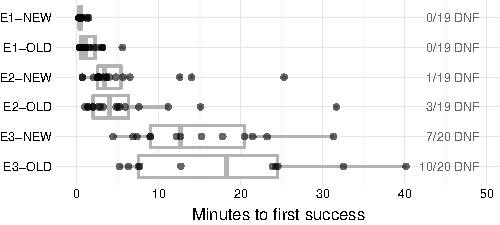
\includegraphics{time_to_success}
\caption{
Time to first success, by censorship environment and interface.
The dots show the raw completion times;
while the boxplots show the medians and interquartile ranges.
The ``DNF'' figures at the right
show the number of participants who did not finish
in the time alloted.
}
\label{fig:time_to_success}
\end{figure}

\begin{figure}
\centering
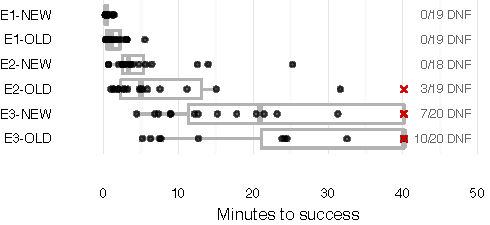
\includegraphics{time_to_success_clamped}
\caption{
Time to first success, by censorship environment and interface.
Here, non-finishing participants are assigned a time of 40 minutes.
}
\label{fig:time_to_success_clamped}
\end{figure}

\begin{figure}
\centering
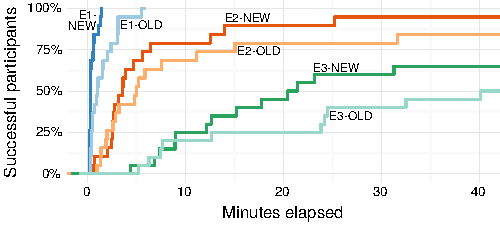
\includegraphics{time_to_success_ecdf}

% Generated by info.R:
\begin{tabular}{l r r r r}
& \multicolumn{1}{c}{1.5~m} & \multicolumn{1}{c}{10~m} & \multicolumn{1}{c}{20~m} & \multicolumn{1}{c}{40~m} \\
\noalign{\hrule}
E1-NEW & 100\% & 100\% & 100\% & 100\% \\
E1-OLD & 58\% & 100\% & 100\% & 100\% \\
E2-NEW & 11\% & 79\% & 89\% & 95\% \\
E2-OLD & 16\% & 68\% & 79\% & 84\% \\
E3-NEW & 0\% & 25\% & 45\% & 65\% \\
E3-OLD & 0\% & 20\% & 25\% & 50\% \\
\end{tabular}

\caption{
Cumulative success rates over time.
We stopped participants after 40 minutes;
this graph shows what the success rate would have been
at different cutoff times.
For example, every E1-NEW participant finished within 90 seconds,
but only 58\% of E1-OLD had finished by that time.
After 10 minutes, 79\% of E2-NEW and 68\% of E2-OLD had finished.
After 20 minutes, 45\% of E3-NEW and only 25\% of E3-OLD had finished.
}
\label{fig:time_to_success_ecdf}
\end{figure}

{\color {red} 
What to talk about: 
\begin{itemize}
\item{Did the new interface improve the success rate?}
\item{Did the new interface help in only certain environments or certain people?}
\item{Did the new interface improve the time to success?}
\item{What are remaining issues?} 
\item{What people did while configuring the interface}
\item{Where people downloaded Tor browser if they did it themselves} 
\item{Xlab versus craigslist} 
\end{itemize} 

Graph: 
\begin{itemize}
\item{success rate}
\item{time spent on each screen}
\item{order pluggable transports were chosen}
\item{transitions between windows for all participants}
\end{itemize} 
} 

\section{Limitations} 
The interface was only tested on windows machines, which were the only types of machines available machines in Xlab. The configuration interface uses the native operating system's elements and their respective styling, so an interface looks slightly different across different operating systems. Participants who are not accustomed to using Windows machines may have been slower than usual to complete the given task, but this effect should affect all of our conditions equally. 

Our study was conducted in an inorganic setting, which can cause our participants to be under or over-motivated. Our participants had a monetary incentive  to connect to Tor, whereas as a real user in a censored environment would Tor to reach a particular website or service. Additionally, the presence of researchers may have placed social pressure to attempt connect for the whole duration of the session, when they would have given up if they were not in a laboratory setting.   

We did not test cases in which the user is required to configure a custom bridge or proxy. Our participants were from one geographic location in the United States and are able to speak English.

\section{Future Work} 
Throughout the qualitative user study, redesign of the interface, and the quantitative user study, we collaborated and communicated with Tor developers. Redesigning the configuration interface was a mutual interest. In fact, Tor version {\color{red} 5.?.?} incorporated textual and navigational changes based on our redesigned interface. We plan to continue our work with Tor developers to integrate changes we found to be helpful. This process will entail debugging our code, merging changes with the current version of Tor, making high-fidelity graphics that align with style guides, and finalizing the advice to give to users in the interface. 

Ideally, we want users in censorship environments across the world to succeed in connecting to the Tor network in a couple of minutes. Currently, the deployed nor redesigned interface achieves this goal. Additional user studies that focus specifically on users in heavily censored environments, or increasing the amount of automation in the configuration process can yield to higher rates of success and faster time to success. We encourage future work to explore some of the non-conservative changes and alternative approaches that we were not able to test in these series of experiment, which are listed in Section~\ref{sec:discussion}. 

\section{Discussion} 
\label{sec:discussion}
If we had more concrete information on the number of high-risk users or users who need to configure a proxy, we would have made additional changes in the prototype. Since we lacked this information, the following changes did not make it into our prototype, but are worth discussing. Depending on the number of high-risk users or proxy-configuring users, these additional changes may be helpful: \\

\begin{itemize}
\item {\bfseries Tell people to click connect.} On the first screen, the user needs to decide to connect or configure. Although there is a description of what each option entails and when one may consider using that option, there are no instructions for the user on what to do. Ideally, we would people to click connect, and then try the manual configuration if a direct connection fails. We currently do not communicate this because it may put some users at risk. However, it is believed that a majority of the users will succeed if they click connect on the first screen, and giving them instructions on what to do can lessen their cognitive load during the configuration process. 
\item{\bfseries Hide the proxy screen.} Don't give users the option to configure a proxy unless it has been detected that it would be necessary. The amount of people who use proxies is low, but then \ldots this would not give users control in the beginning of the configuration process. 
\item{\bfseries Help the at-risk users.} There are people who would benefit from, on the first attempt, connecting with a meek bridge or custom bridge, without trying a vanilla tor connection or the recommended bridge in the dialog. Currently, we guide these people to the correct decision, but after trying the default bridge first. Helping these users to make a connection safely without ever being logged as connecting to Tor would be a benefit, but might be a case of overfitting to these types of users. A majority of users should not use a meek bridge or custom bridge, so it would be unideal to lead all users to this decision.
\end{itemize} 

We took an approach that optimized for the average case user yet was conservative in automation to allow at-risk users to possibly connect without leaking that they use Tor. We believe that this is a sound approach to interacting with the user and the one we would recommend personally. However, there are alternative approaches to interacting with the user that may be of interest: \\

\begin{itemize}
\item{\bfseries Automate the entire configuration process.} This sounds like a radical idea, but it really isn't. Today, this wouldn't harm most of our users. Our study finds that most users do not configure better than we do and would leak that they are using Tor anyway. 
\item {\bfseries Auto-configure after connect.} After a person has already clicked connect and the connection was unsuccessful, they have already been logged. I am assuming that the significant difference is between being logged trying to connect to Tor or not at all, rather than the number of connection attempts made. This would greatly save our users a lot of headache. 
\item{\bfseries Ask about the risk.} Rather than having the configuration dialog be manual by default, just ask if the users are at risk if the process was automated. If they are not at risk, we can do it automatically, and the at-risk users can configure manually. The issue with this is that people may not answer this question honestly, or they might not know the correct answer to this question. 
\item{\bfseries Ask if they are qualified to make decisions.} Asking users if they know which bridge to choose, and choosing for them if they say they don't know. We probably know better than they do. But there are ethical implications of choosing bridges for them rather them making the mistakes themselves. The issue with this is that people may not answer honestly. 
\end{itemize}

\section {Acknowledgments}
{\color {red} Rowilma del Castillo for setting up Xlab, Nima Fatemi, Isabella Bagueros, Georg Koppen, and the UX team for giving feedback, and Cecile Basnage for reviewing the UI of circumvention tools.} 
{\color {red} Tor Browser devs for taking our recommendations to heart and implementing changes.}

\section{Conclusion} 
{\color {red} I am a fan of not having long, rambling conclusions. I leave
that for the discussion section. This section is more of a courtesy to the 
people who read the abstract, look at the figures, and then read the 
conclusion. Think of something to tell those people here. Something along
the lines of a tl;dr summary of the paper.} 

\bibliographystyle{abbrv}
\nocite{*}
\bibliography{pets2017-paper}

\appendix
\section{Participant Worksheet Text} 
\label{participant-worksheet}
Imagine you live in an oppressive country that censors part of the Internet. We have simulated this in the laboratory by blocking certain websites and services. The purpose of this experiment is to evaluate the use of Tor browser, which is a browser that can circumvent censorship and let you visit blocked websites. For instance, www.torproject.org is blocked. Check this by going to the site on a standard browser, like Firefox, Chrome, or Internet Explorer. It will fail to load, when you can visit other sites.

To complete this worksheet, you will need to set up Tor browser (on your desktop) correctly and use it to get to blocked site. If you can visit wikipedia, then you know that you have successfully circumvented censorship.

\section{Qualitative User Study Recruitment Posting} 
\label{qualitative-recruitment}
We are recruiting participants for an in-person research study at the University of California, Berkeley. You will need to come in to our lab and perform tasks on a computer for an hour or less. You will be compensated \$30 for participating. 
No special knowledge and no technical experience is required. If you are interested, fill out the survey at \textit{<survey link>}. 

\section{Qualitative User Study Prescreening Survey} 
\label{qualitative-prescreening}
We are recruiting participants for an in-person research study at the University of California, Berkeley. You will need to come in to our lab and perform tasks on a computer for an hour or less. You will be compensated \$30 for participating. No special knowledge and no technical experience is required.\\

\begin{enumerate}
\item{Please select when you are available. We will assign you an hour experiment time slot during one of those times.}
\item{I am able to provide my own transportation to the University of California, Berkeley campus.}
\item{Thank you for your interest! Please provide an email address where we can contact you to share more logistical details.}
\item{we are looking for a very small number of participants, so unfortunately, we may not be able to accommodate everyone who applies. Would you like us to let you know about future opportunities?}
\item{What is your gender?}
\item{What is your age?}
\item{Please select your highest completed (or current) level of education.}
\item{What is your occupation?} 
\item{Do you speak any languages other than English fluently?}
\item{If you have a personal computer, what kind do you use?}
\item{Which of the following terms have you heard of? \textit{<answer choices: a checkboxlist of the the following terms: malware, proxy services, phishing, SSL, X.511 certificates, Tor>}}
\item{How often do you use the following software or features? \textit{<answer choices: a grid of radio buttons. Software/features (rows): HTTPS on web pages, proxies or other censorship circumvention tools, virtual private networks (VPN), file or whole-disk encryption, anonymity systems (e.g., Tor), email encryption (e.g., PGP), chat or instant messaging encryption, voice communication encryption. Frequency (columns): never, less than once a month, a few times a month, several times a week, daily.>}}
\end{enumerate}
Thank you for filling out this form. You are now done!

\section{Qualitative User Study Introduction Script} 
\label{qualitative-script} 
Imagine you live in an oppressive country that censors part of the Internet. We have simulated this in the laboratory by blocking certain websites and services.  The purpose of this experiment is to evaluate the use of Tor browser, which is a browser that can circumvent censorship and let you visit blocked websites. Currently, torproject is blocked (you can check this by going to torproject.org on a standard browser, like Firefox, Chrome, or Internet Explorer). 

To circumvent censorship successfully, you will need to set up Tor browser correctly and use it to get to Wikipedia. If you are able to reach the website, then you know that you have successfully circumvented censorship. Fill out the question on the worksheet. This isn't intended to be hard, just write what you see. We want to just check you saw the website. 

Before you start, do you have any questions about what you are asked to do? 

\section{Post-Experiment Standard Interview Questions}
We asked our participants these questions after they were given time to configure Tor Browser. \\

\begin{enumerate}
\item{Can you talk us through what you did along with what you were thinking at the time?}
\item{What was most challenging part of connecting?}
\item{Were there any unfamiliar terms?}
\item{How did you decide which options to choose?}
\item{What did you think about using Tor?}
\item{What is one change you would recommend?} 
\item{Did you need any additional information?} 
\end{enumerate}  

In addition to these questions, we asked our participants about specific questions based on their observation, usually regarding a specific choice in action, a particular screen they seemed stuck on, and any errors they encountered during the configuration process. 

\section{Quantitative User Recruitment Posting}
\label{quantitative-recruitment}
We are recruiting up to 40 participants for a user study at UC Berkeley. The experiment will involve basic Internet browsing tasks. You are not eligible if you have participated in our previous sessions.\\

\indent Payment: \$30 Amazon gift card\\
\indent Duration: 1 hour \\
\indent Where: Xlab at Hearst Memorial Gymnasium\\

\textit{<list of sessions>}\\

To be eligible, you must be an adult (18 or older). This is to comply with university policies on research. 

If you are interested: 1. Email lnl@berkeley.edu with the sessions you are able to attend. We will confirm your participation and assign you a session. 2. Come to Xlab at the appointed time for the experiment.

\section{Quantitative User Study Introduction Script} 
\label{quantitative-script} 
Imagine you live in an oppressive country that censors part of the Internet. We have simulated this in the laboratory by blocking certain websites and services.  The purpose of this experiment is to evaluate the use of Tor browser, which is a browser that can circumvent censorship and let you visit blocked websites. Currently, torproject is blocked (you can check this by going to torproject.org on a standard browser, like Firefox, Chrome, or Internet Explorer). 

To circumvent censorship successfully, you will need to set up Tor browser correctly and use it to get to Wikipedia. If you are able to reach the website, then you know that you have successfully circumvented censorship. Fill out the question on the worksheet. This isn't intended to be hard, just write what you see. We want to just check you saw the website. 

Afterward, we ask you to take a short survey to collect some information about you. The link is also on your worksheet.
We will give you time to complete this task. If you finish early, we ask that you sit at your desk until the remainder of the hour. Since we are recording your screen, we ask that you don't do anything personal afterward, like checking your email.

Before you start, do you have any questions about what you are asked to do? 

\section{Quantitative User Study Exit Survey} 
\label{quantitative-exit-survey}
We'd like to know more about you.  All of your answers will be stored separately from any identifying information in order to protect your confidentiality.

This survey is part of a research project being conducted by the University of California, Berkeley. If you have any questions about your rights or treatment as a research participant in this study, please contact the University of California at Berkeley's Committee for Protection of Human Subjects at 510-642-7461, or email subjects@berkeley.edu. If you agree to participate, please click Next below.\\

\begin{enumerate}
\item{What is your participant ID? (This can be found on the sticker ont he left hand corner of the desk you are currently sitting at.)}
\item{What is your gender?}
\item{What is your age?}
\item{Please select your highest completed (or current) level of education}.
\item{What is your current occupation?}  
\end{enumerate}

Thank you for participating in our experiment. You are now done! Please sit at your desk for the remainder of the experiment. Our researchers will formally announce the end of the experiment. 
\end{document}
